%------------------------------------------------
% talk.tex - slides for DjangoCon 2015
%------------------------------------------------
\documentclass[screen]{camel}

% options (these don't work!)
% \cymraegtrue
% \screentrue
% \booklettrue
% \blankstrue
% \answerstrue

% module information
%\academicyear{2015-16}
%\modulecode{MA0000}
%\moduletitle{Cardiff Maths e-Learning}

\academicyear{}
\modulecode{}
\moduletitle{}

%
%\booknumber{1}
%\booktitle{User Guide}
%\bookauthor{Dafydd Evans}
%\bookversion{v0.1}

% figures
\usepackage{graphicx}
\graphicspath{{./figures/}}
\DeclareGraphicsExtensions{.pdf,.jpg,.png,.gif}
\usepackage{caption}
\usepackage{subcaption}
\captionsetup[subfigure]{labelformat=empty}
\captionsetup[figure]{skip=2ex}

% naughty
\def\it{\item}
\def\bit{\begin{itemize}}
\def\eit{\end{itemize}} 
\def\ben{\begin{enumerate}}
\def\een{\end{enumerate}}

% macros
\newcommand{\Z}{\mathbb{Z}}
\newcommand{\N}{\mathbb{N}}
\newcommand{\R}{\mathbb{R}}
\newcommand{\C}{\mathbb{C}}

% parallel columns (en/cy)
\usepackage{paracol}

\usepackage{titlesec}
%\sethead{}{}{\scriptsize DjangoCon Europe 2015}
%\setfoot{\scriptsize D Evans}{\scriptsize Cardiff School of Mathematics}{\scriptsize\thepage}

\renewpagestyle{slides}[\tiny\scshape]{
	\sethead{}{}{\scriptsize DjangoCon Europe 2015}
	\footrule
	\setfoot{\scriptsize D Evans}{\scriptsize Cardiff School of Mathematics}{\scriptsize\thepage}
}
\pagestyle{slides}

\assignpagestyle{\chapter}{slides}

% Default fixed font does not support bold face
\DeclareFixedFont{\ttb}{T1}{txtt}{bx}{n}{12} % for bold
\DeclareFixedFont{\ttm}{T1}{txtt}{m}{n}{12}  % for normal

% Custom colors
\usepackage{color}
\definecolor{deepblue}{rgb}{0,0,0.5}
\definecolor{deepred}{rgb}{0.6,0,0}
\definecolor{deepgreen}{rgb}{0,0.5,0}

\usepackage{textcomp}
\usepackage{listings}
%\usepackage{courier}


% python code
\newcommand\pythonstyle{\lstset{
language=Python,
basicstyle=\ttfamily\scriptsize,
breaklines=true,
upquote=true,
otherkeywords={self},             % Add keywords here
keywordstyle=\ttb\color{deepblue},
emph={MyClass,__init__},          % Custom highlighting
emphstyle=\ttb\color{deepred},    % Custom highlighting style
stringstyle=\color{deepgreen},
morekeywords={MPTTModel,TreeForeignKey,CharField,PositiveSmallIntegerField,TextField},
showstringspaces=false            % 
}}
% latex code
\newcommand\latexstyle{\lstset{
language=[LaTeX]TeX,
basicstyle=\ttfamily\scriptsize,
%texcsstyle=*\color{blue},
keywordstyle=\color{blue},
%otherkeywords={$, \{, \}, \[, \]},
%otherkeywords={maketitle},
morekeywords={maketitle,chapter, question, choice, correctchoice},
commentstyle=\color{red},
tabsize=2
}}
% html code
\newcommand\htmlstyle{\lstset{
language=HTML,
basicstyle=\ttfamily\scriptsize,
keywordstyle=\color{blue},
commentstyle=\color{red},
otherkeywords={equation},
tabsize=2
}}
% xml code
\newcommand\xmlstyle{\lstset{
language=XML,
basicstyle=\ttfamily\scriptsize,
morestring=[b][\color{red}]",
keywordstyle=\color{blue},
commentstyle=\color{red},
%identifierstyle=\color{cyan},
morekeywords={xml-stylesheet,book,chapter,section,homework,question,questions,answer,ref,jax},
%frame=single,
tabsize=2
}}

% listings environments
\lstnewenvironment{python}[1][]{\pythonstyle\lstset{#1}}{}
\lstnewenvironment{latex}[1][]{\latexstyle\lstset{#1}}{}
\lstnewenvironment{html}[1][]{\htmlstyle\lstset{#1}}{}
\lstnewenvironment{xml}[1][]{\xmlstyle\lstset{#1}}{}

% tweaks
\addtolength{\tabcolsep}{0.5ex}
\renewcommand{\arraystretch}{1.1}
\addtolength{\arraycolsep}{0.5ex}

\newcommand{\rmTeX}{\textrm{\TeX\ }}
\newcommand{\rmLaTeX}{\textrm{\LaTeX\ }}

% tikz
\definecolor{djangogreen}{RGB}{9,46,32}
\usepackage{tikz}
\usetikzlibrary{shapes.geometric, arrows}


% camel logo
\makeatletter
%\def\p@CaMeL{{\reset@font\rm C\kern-.20em%
%    \raise.4ex\hbox{\sc a}\kern-.15em%
%    M\kern-.1667em\lower.7ex\hbox{E}\kern-.125emL}}
\def\p@CaMeL{{\reset@font\rm C\kern-.20em%
    \raise.4ex\hbox{\sc a}\kern-.15em%
    M\kern-.1667em\lower.7ex\hbox{E}\kern-.125emL}}
\def\CaMeL{\protect\p@CaMeL}  
\makeatother


\makeatletter
\pgfarrowsdeclare{crow's foot}{crow's foot}
{
  \pgfarrowsleftextend{+-.5\pgflinewidth}%
  \pgfarrowsrightextend{+.5\pgflinewidth}%
}
{
  \pgfutil@tempdima=1.2pt%
  \advance\pgfutil@tempdima by.25\pgflinewidth%
  \pgfsetdash{}{+0pt}%
  \pgfsetmiterjoin%
  \pgfpathmoveto{\pgfqpoint{0pt}{-6\pgfutil@tempdima}}%
  \pgfpathlineto{\pgfqpoint{-6\pgfutil@tempdima}{0pt}}%
  \pgfpathlineto{\pgfqpoint{0pt}{6\pgfutil@tempdima}}%
  \pgfusepathqstroke%
}
\makeatother

%------------------------------------------------
\begin{document}
%\makefrontmatter
    \thispagestyle{empty}
\mbox{}\vfill
\begin{center}
	\scshape
	\Huge \CaMeL \\[1ex]
	\huge {\normalfont The Cardiff Maths eLearning Project} \\[4ex]
	\large Dafydd Evans \\
	\normalsize Cardiff School of Mathematics\\[4ex]
	\large DjangoCon Europe \\
	 \normalsize 1st June 2015
\end{center}
%\vfill\mbox{}
\normalsize

%------------------------------------------------
%\chapter*{Outline}\label{ch:outline}
%------------------------------------------------
\setcounter{tocdepth}{0}
\tableofcontents
%%------------------------------------------------
%\chapter{Introduction}\label{ch:intro}
%%------------------------------------------------
%\ben
%\it Introduction
%	\ben
%	\it Motivation
%	\it Typesetting Guttenberg, markup/tagging, author->printer) FIG: type-trays
%	\it HTML FIG: latex2html | mathjax
%	\it \LaTeX (history, fonts, structure) CODE: html | latex
%	\it \LaTeX commands/environments; levels, boxes, theorems, lists, items, figures; 
%	\it camel.cls with switches, extends book.cls and exam.cls, FIG: noblanks | blanks
%	\een
%\it LatexTree
%	\ben
%	\it well-formedness (xml), regular/fsa and context-free/pda
%	\it algorithm inc levels, \verb+parse_block+, labels
%	\it recursive output: materialised path tree, xml|database FIG: xml screenshot
%	\een
%\it Django
%	\ben
%	\it system diagram
%	\it models: basic BookNodes subclassess MPTTNode; mptt package/tags
%	\it database diagram
%	\it latex environments for interaction (compare edx.sty)
%	\it data
%	\een
%\it Future work
%	\ben
%	\it functional, technical
%	\een
%\een
%
%BLAH

%------------------------------------------------
\chapter{Motivation}\label{ch:motivation}
%------------------------------------------------
Writing mathematics requires specific layouts and fonts.


\ben
\it Learning materials.
	\bit  
	\it Teachers produce high-quality PDF documents using \LaTeX.
	\it PDF documents lack interactive capabilities.
	\eit
\it Homework submission and feedback.
	\bit
	\it Students submit handwritten solutions to homework questions.
	\it Teachers marks and returns the scripts
	\eit
\een

%Possible solutions:
%\bit
%\it Student submits a scanned copy of handwritten work.
%\it Student prepares an Microsoft Word file. 
%\it Student prepares a PDF file using the \LaTeX\ typesetting system. 
%\eit
%
%\bit
%\it MSWord is a non-starter: time-consuming and ugly mathematical fonts.
%\it \TeX\ and \LaTeX\ state-of-the-art
\begin{mdframed}
\begin{center}
\vspace*{1ex}
Can \LaTeX\ documents be used as the basis of an e-learning system for mathematics?
\vspace*{1ex}
\end{center}
\end{mdframed}

%------------------------------------------------
\chapter{Typesetting}\label{ch:typesetting}
%------------------------------------------------
\columnratio{0.6}
\begin{paracol}{2}
\bit
% ka-NOOTH
\it Basic building blocks are letters, numerals and symbols. These are collectively known as \emph{glyphs}.
\it Groups of glyphs are called \emph{fonts}.
\it Groups of fonts sharing particular design features are called \emph{typefaces}.
\it Computer Modern typefaces for mathematics created by Donald Knuth for \TeX\ (1978)
\it \TeX\ extended to \LaTeX\ by Leslie Lamport (1984).
\it \LaTeX\ is the de-facto standard for typesetting mathematical articles and books.
\eit

\switchcolumn
\raggedleft
\resizebox{0.35\textwidth}{!}{\includegraphics{moveable_type_chinese}} 
%\resizebox{0.35\textwidth}{!}{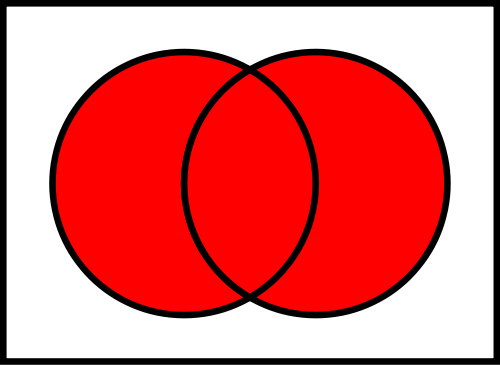
\includegraphics{AcupB}}
\par\bigskip
\resizebox{0.35\textwidth}{!}{
\includegraphics{moveable_type_english}}
%\resizebox{0.35\textwidth}{!}{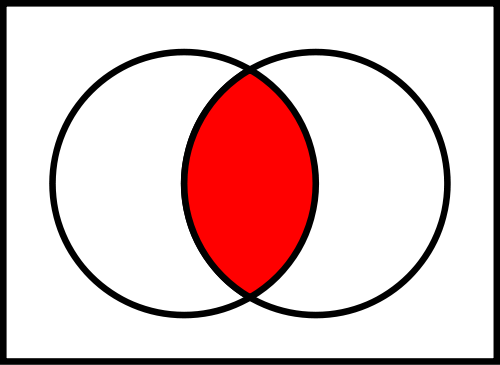
\includegraphics{AcapB}}
\end{paracol}

%%------------------------------
%\slidebreak
%\section{TeX and LaTeX}
%%------------------------------
%\bit
%\it $\tau\epsilon\chi\nu\eta$ (techn\'{e}), Greek for ``art, craft, skill'', 
%\it TeX - > DVI (screen) PS (paper)
%\it TeX commands start with a backslash and are grouped with curly braces.
%\eit

%------------------------------
\slidebreak
\section{Mark-up Languages}
%------------------------------
%\lstset{language=[LaTeX]TeX,
%    basicstyle=\ttfamily\scriptsize,
%%    texcsstyle=*\color{blue},
%    keywordstyle=\color{blue},
%    otherkeywords={chapter},
%	tabsize=2
%}
%\lstset{language=HTML,
%    basicstyle=\ttfamily\scriptsize,
%    keywordstyle=\color{blue},
%    commentstyle=\color{red},
%    otherkeywords={equation},
%    tabsize=2
%}

\begin{tabular}{|p{0.45\textwidth}|p{0.45\textwidth}|} \hline

\texttt{LaTeX -> PDF} & \texttt{HTML -> Web} \\ \hline

\begin{latex}
\documentclass{book}
	\title{My Book}
\begin{document} %comment
	\maketitle
	\chapter{Introduction}
	Hello world.
	\begin{equation}\label{eq:gauss}
		\int_{-\infty}^{+\infty} 
			e^{-x^2}dx = \sqrt{\pi}.
	\end{equation}
\end{document}
\end{latex}

& 

\begin{html}
<html>
	<head>
		<title>My Book</title>
	</head>
	<body> <!-- comment -->
		<h1>Introduction</h1>
		Hello world!
		<equation id="eq:gauss">
			oops!
		</equation>
	</body>
</html>
\end{html}

\\ \hline
\end{tabular}
\vfill
\bit
\it Mark-up used to define \emph{structure}, \emph{styles}, \emph{cross-references} and \emph{citations}.
\it \LaTeX\ documents are not ``well-formed''.
%\it xml schema: \texttt{DocBook} and \texttt{MathML}.
%\it \texttt{MathJax} can render mathematical fonts in web browsers.
\eit
\vfill
%------------------------------
\slidebreak
\section{\rmLaTeX}
%------------------------------
\columnratio{0.5}
\begin{paracol}{2}

%\begin{tabular}{ll}
%Level		& \texttt{book, chapter, section, subsection} \\
%Theorem	& theorem, lemma, \\
%Float		& figure, table, ..
%\end{tabular}

%\underline{Structural}
\subsection*{Structural mark-up}
\small
%\textsl{Structural mark-up}
\verb+\chapter,\section,...+ \\
%\verb+equation,theorem,...+ \\
%\verb+\begin{env}...\end{env}+
\verb+\begin{equation}...\end{equation}+
%\verb+\begin{equation}+ \\
%\mbox{}\quad\verb+...+ \\
%\verb+\end{equation}+
\normalsize
%\bit
%\it \verb+\chapter,\section,...+
%\it \verb+\definition,\theorem,...+
%\eit
%\vfill
%\textsl{Stylistic mark-up}
\subsection*{Stylistic mark-up}
\small
\verb+\textbf,\textit,...+ \\
\verb+\alpha,\pi,\partial,...+
\normalsize
%\bit
%\it \verb+\textbf,\textit,...+
%\it \verb+\alpha,\pi,\partial,...+
%\eit
%\vfill
%\textsl{Cross-references and citations}
\subsection*{Cross-references and citations}
\small
\verb+\label,\ref,\cite.+
\normalsize
%\bit 
%\it \verb+\label,\ref,\cite.+
%\eit
%And ...
%\bit
%\it Scalable mathematical fonts.
%\it Automatic numbering
%\it Cross-references and citations.
%	\bit 
%	\it \verb+\label+, \verb+\ref+ and \verb+\cite+.
%	\eit
%\eit
%\vfill
%\textsl{Extensible}
\subsection*{Extensible}
\small
\verb+\begin{homework}...\end{homework}+ \\
\verb+\question+
%\verb+exam.cls+ by Phil Hirschhorn (MIT) \\
%\verb+camel.cls+ by DE (CU).
\normalsize
%\bit
%\it \verb+exam.cls+ by Phil Hirschhorn.% (MIT)
%%\it \verb+camel.cls+ by DE.
%\eit

\switchcolumn

\begin{latex}
\documentclass{camel}
	\title{Lecture Notes}
\begin{document} 
	\maketitle
	\chapter{Introduction}\label{ch:intro}
	Hello world.
	\begin{equation}\label{eq:gauss}
		\int_{-\infty}^{+\infty} 
			e^{-x^2}dx = \sqrt{\pi}.
	\end{equation}
	\chapter{Background}
		In Chapter~\ref{ch:intro} we saw ...
		\begin{homework}
			\begin{questions}
				\question Area of a circle?
				\begin{answer}
				$A = \pi r^2$
				\end{answer}
			\end{questions}
		\end{homework}
\end{document}
\end{latex}

\end{paracol}


%------------------------------
\slidebreak
\section{Yet Another \textrm{\LaTeX\ }Parser}\label{sec:booktree}
%------------------------------
\vfill
\bit
\it Implemented in python.
\it Source file processed using regular expressions and a stack (pushdown automaton).
\it Output is a so-called \emph{materialized path tree}.% representation of the document.
\it Numbering implemented using class variables.
\it Mathmode environments/commands left for \textcolor{deepred}{\texttt{MathJax}} to handle.
\eit
\vfill
\begin{python}
latex_node_types = {
    'level': ('book', 'chapter', 'section', 'subsection'),
    'theorem': ('definition', 'theorem', 'lemma', 'remark', 'example', 'exercise'),
    'mathmode': ('equation', 'eqnarray', 'array', 'align', 'cases'),
    'list': ('itemize', 'enumerate',  'questions', 'parts', 'subparts', 'choices'),
    'item': ('item', 'question', 'part', 'subpart', 'choice', 'correctchoice'),
    'float': ('table', 'figure', 'subtable', 'subfigure'),
    'box': ('proof', 'solution', 'answer', 'hint'),
    'assignment': ('homework', 'mctest'),
    'content': ('jax', 'image', 'reference', 'citation'),
}
\end{python}

%------------------------------
\slidebreak
%\section{Materialized Path Trees}
%------------------------------
%<?xml version="1.0" ?>
%<?xml-stylesheet type="text/css" href="camel.css"?>
%Sample XML output:
\begin{xml}
<book>
  <chapter label="ch:intro" number="1" title="Introduction">
    <jax>Hello world. 
\begin{equation}
\int_{-\infty}^{+\infty} e^{-x^2}dx = \sqrt{\pi}.
\end{equation}</jax>
  </chapter>
  <chapter number="2" title="Background">
    <jax>In Chapter </jax>
    <ref target="ch:intro">1</ref>
    <jax>we saw ...</jax>
    <homework number="1">
      <questions number="1">
        <question number="1">
          <jax>Area of a circle?</jax>
          <answer>
            <jax>$A = \pi r^2$</jax>
          </answer>
        </question>
      </questions>
    </homework>
  </chapter>
</book>
\end{xml}

%------------------------------------------------
%\chapter{Cardiff Maths eLearning (Camel)}\label{ch:django}
%\chapter[The Cardiff Maths eLearning Project]{\CaMeL\ -- \normalfont The Cardiff Maths eLearning Project}\label{ch:django}
%\chapter[The Cardiff Maths eLearning Project]{\CaMeL\ --\normalfont The Cardiff Maths eLearning Project}\label{ch:django}
\chapter[The Cardiff Maths eLearning Project]{The \CaMeL\ project}\label{ch:camel}
%------------------------------------------------
\tikzstyle{nobox} = [minimum width=10ex, minimum height=4ex,text centered, draw=none]
\tikzstyle{basic} = [rectangle, rounded corners, minimum width=12ex, minimum height=5ex,text centered, draw=black]
\tikzstyle{django} = [rectangle, rounded corners, minimum width=12ex, minimum height=5ex, text centered, draw=black, fill=deepgreen!30]
\tikzstyle{arrow} = [ultra thick,->,>=latex]

\begin{tikzpicture}[font=\ttfamily, node distance=10ex]
\node (pdf) [nobox] {pdf};
\node (xml) [nobox, right of=pdf, xshift=7ex] {xml};
\node (latex) [basic, fill=yellow!20, below of=pdf] {\texttt{latex}};
\node (doctree) [basic, fill=blue!10, right of=latex, xshift=7ex] {doctree};
\node (models) [django, right of=doctree, xshift=7ex] {models};
\node (database) [basic, fill=red!20, right of=xml, xshift=15ex] {database};
\node (views) [django, right of=models, xshift=7ex] {views};
\node (templates) [django, right of=views, xshift=7ex] {templates};
\node (web) [nobox, right of=database, xshift=16ex] {web};
\draw [arrow] (latex) -- (doctree);
\draw [arrow] (latex) -- (pdf);
\draw [arrow] (doctree) -- (xml);
\draw [arrow] (doctree) -- (models);
\draw [arrow] (models) -- (database);
\draw [arrow] (database) -- (views);
\draw [arrow] (views) -- (templates);
\draw [arrow] (templates) -- (web);
\end{tikzpicture}

\vspace*{2ex}
\subsection*{Models}
\ttfamily
\bit
\it \verb+BookNode: node_type, number, title, content, mpath+
\it \verb+Label: label_text, target_mpath+
\it \verb+Answer: user, question, text+
%\it \verb+MultipleChoiceAnswer: user, question, choice+
\it \verb+Submission: user, assignment+
\eit
\normalfont

\vfill\hfill\small\textcolor{deepgreen}{\texttt{http://github.com/dimbyd/camel/}}\normalsize
%------------------------------
\slidebreak
\section{\texttt{django-mptt}}
%------------------------------
\raggedright
Modified Preorder Tree Traversal (MPTT) is a technique for storing and accessing hierarchical data in a database. 
\bit
\it Retrieval operations are efficient.
\it Inserts, moves and deletions are comparatively expensive.
\eit

\vspace*{1.5ex}
The \textcolor{blue}{\texttt{django-mptt}} app makes it very easy to use MPTT with Django models.
\bit
%\it Handles the details of managing database tables as tree structures.
%\it Provides tools for working with trees of model instances.
\it Models are defined as subclasses of \verb+mptt.models.MPTTModel+.
%\bit
%\it Fields required for tree structure are added automatically.
%\eit
\it Tree updated automatically when model instances are inserted/moved/deleted.
%\it Tree structure updated automatically when model instances are inserted/moved/deleted.
\it Instance methods: \verb+get_ancestors()+, \verb+get_children()+, etc.
\it Custom form fields provided by the \verb+mptt.forms+ package.
\it Template tags and filters for rendering trees recursively.
\eit

\vfill\hfill\small\textcolor{deepgreen}{\texttt{http://github.com/django-mptt/django-mptt/}}\normalsize

\slidebreak

\subsubsection*{\texttt{models.py}}\vspace*{-1ex}
\begin{python}
class BookNode(MPTTModel):
    parent = TreeForeignKey('self', null=True, related_name='children')
    node_type = models.CharField(max_length=10)
    number = PositiveSmallIntegerField(null=True)
    title = CharField(max_length=100, null=True, blank=False)
    content = TextField(null=True)
    mpath = CharField(max_length=100, null=True)
\end{python}

\vspace*{1ex}
\subsubsection*{\texttt{views.py}}\vspace*{-1ex}
\begin{python}
context['chapter'] = BookNode.objects.get( pk=pk )
context['subtree'] = context['chapter'].get_descendants(include_self=True)
\end{python}

\vspace*{1ex}
\subsubsection*{\texttt{template.html}}\vspace*{-1ex}
\begin{html}


	
		<div class="chapter">
			<h1 class="chapter">{{ node.number }}. {{ node.title }}</h1>
			{{ children }}
		</div>
	 ...
\end{html}


%------------------------------
\slidebreak
\section{Custom \rmLaTeX environments for interaction}
%------------------------------

The following were inspired by \verb+exam.cls+ (written by Phil Hirschhorn, MIT).

\vspace*{2ex}
\columnratio{0.5}
\begin{paracol}{2}

\subsubsection*{Free-text answers}
\begin{latex}
\begin{homework}
	\begin{questions}
	\question
	First Question.
		\begin{solution}
		Solution of First Question.
		\end{solution}
	\question
	Second Question.
		\begin{solution}
		Solution of Second Question.
		\end{solution}
	\end{questions}
\end{homework}
\end{latex}

\switchcolumn

\subsubsection*{Multiple-choice answers}
\begin{latex}
\begin{mctest}
	\begin{questions}
	\question
	Which is the odd one out?
	\begin{choices}
		\choice John
		\choice Paul
		\choice George
		\correctchoice Dingo
	\end{choices}
	\end{questions}
\end{mctest}
\end{latex}

\end{paracol}

%------------------------------
\slidebreak
\section{Database schema}
%------------------------------
\tikzstyle{basic} = [rectangle, rounded corners, minimum width=15ex, minimum height=5ex,text centered, draw=black]
%\tikzstyle{django} = [rectangle, rounded corners, minimum width=12ex, minimum height=5ex, text centered, draw=black, fill=deepgreen!30]
\tikzstyle{arrow} = [thick,-,>=latex]
\vfill
\begin{center}
\begin{tikzpicture}[font=\ttfamily, node distance=10ex]
\node (student) [basic, fill=green!10] {student};
\node (module) [basic, fill=red!10, right of=student, xshift=15ex] {module};
\node (book) [basic, fill=blue!10, right of=module, xshift=15ex] {book};
\node (submission) [basic, fill=green!10, below of=student, yshift=-5ex] {submission};
\node (homework) [basic, fill=blue!10, below of=module, yshift=-5ex] {homework};
\node (answer) [basic, fill=green!10, below of=submission, yshift=-5ex] {answer};
\node (question) [basic, fill=blue!10, below of=homework, yshift=-5ex] {question};
%\node (doctree) [basic, fill=blue!10, right of=latex, xshift=7ex] {doctree};
%\node (models) [django, right of=doctree, xshift=7ex] {models};
%\node (database) [basic, fill=red!20, right of=xml, xshift=15ex] {database};
%\node (views) [django, right of=models, xshift=7ex] {views};
%\node (templates) [django, right of=views, xshift=7ex] {templates};
%\node (web) [nobox, right of=database, xshift=16ex] {web};
\draw [arrow] [thick, crow's foot-crow's foot] (student) -- (module);
\draw [arrow] [-crow's foot] (module) -- (book);
\draw [arrow] [-crow's foot] (student) -- (submission);
\draw [arrow] [-crow's foot] (submission) -- (answer);
\draw [arrow] [-] (submission) -- (homework);
\draw [arrow] [-crow's foot] (module) -- (homework);
\draw [arrow] [-crow's foot] (homework) -- (question);
\draw [arrow] [-crow's foot] (question) -- (answer);
%\draw [arrow] (latex) -- (pdf);
%\draw [arrow] (doctree) -- (xml);
%\draw [arrow] (doctree) -- (models);
%\draw [arrow] (models) -- (database);
%\draw [arrow] (database) -- (views);
%\draw [arrow] (views) -- (templates);
%\draw [arrow] (templates) -- (web);
\end{tikzpicture}
\end{center}
\vfill\mbox{}
%------------------------------------------------
\chapter{Next steps}\label{ch:nextsteps}
%------------------------------------------------
\columnratio{0.5}

\begin{paracol}{2}
\subsection*{Django}
\bit
\it Admin pages
\it Teacher pages
\it Visualisation
\it Partial updates using labels
\it PDFs of homework submissions
\it Beautify URLs
\eit

\switchcolumn

\subsection*{Python}
\bit
\it GitHub
\it Exception handling
\it Unit tests
\it Logging
\it \texttt{DocBook} and \texttt{MathML} schemas.
\eit

\end{paracol}

%%------------------------------------------------
%\chapter{Typesetting}\label{ch:typesetting}
%%------------------------------------------------
%\columnratio{0.5}
%\begin{paracol}{2}
%\lstset{language=[LaTeX]TeX, frame=single}
%\texttt{LaTeX}
%\begin{lstlisting}
%\documentclass{book}
%	\title{My Book}
%\begin{document} %comment
%	\chapter{Introduction}
%	Hello world.
%	\begin{equation}
%		\int_{-\infty}^{+\infty} 
%			e^{-x^2}dx = \sqrt{\pi}.
%	\end{equation}
%\end{document}
%\end{lstlisting}
%\switchcolumn
%\texttt{HTML}
%\begin{lstlisting}[language=HTML]
%<html>
%	<head>
%		<title>My Book</title>
%	</head>
%	<body>
%    	<h1>Introduction</h1>
%    	Hello world!
%	</body>
%</html>
%
%\end{lstlisting}
%\end{paracol}
%

%\fbox{\begin{minipage}{0.5\textwidth} lhs \end{minipage}}
%\fbox{\begin{minipage}{0.5\textwidth} rhs \end{minipage}}

%------------------------------------------------
\end{document}
%------------------------------------------------

